%%%%%%%%%%%%%%%%%%%%%%%%%%%%%%%%%%%%%%%%%%%%%%%%%%%%%%%%%%%%%%%%%%%%%%%%%%%
%
% Generic template for TFC/TFM/TFG/Tesis
%
% $Id$
%
% By:
%  + Javier Mac�as-Guarasa.
%    Departamento de Electr�nica
%    Universidad de Alcal�
%  + Roberto Barra-Chicote.
%    Departamento de Ingenier�a Electr�nica
%    Universidad Polit�cnica de Madrid
%
% Based on original sources by Roberto Barra, Manuel Oca�a, Jes�s Nuevo,
% Pedro Revenga, Fernando Herr�nz and Noelia Hern�ndez. Thanks a lot to
% all of them, and to the many anonymous contributors found (thanks to
% google) that provided help in setting all this up.
%
% See also the additionalContributors.txt file to check the name of
% additional contributors to this work.
%
% If you think you can add pieces of relevant/useful examples,
% improvements, please contact us at (macias@depeca.uah.es)
%
% Copyleft 2013
%
%%%%%%%%%%%%%%%%%%%%%%%%%%%%%%%%%%%%%%%%%%%%%%%%%%%%%%%%%%%%%%%%%%%%%%%%%%%

\chapter{Desarrollo hardware}
\label{cha_desarrollo_hardware}

\begin{FraseCelebre}
  \begin{Frase}
No entiendes realmente algo a menos que seas capaz de explic�rselo a tu abuela.    
  \end{Frase}
  \begin{Fuente}
Albert Einstein
  \end{Fuente}
\end{FraseCelebre}


\section{Arquitectura hardware}


\subsection{Plataforma rob�tica base}

\begin{figure}[ht]
\centering
%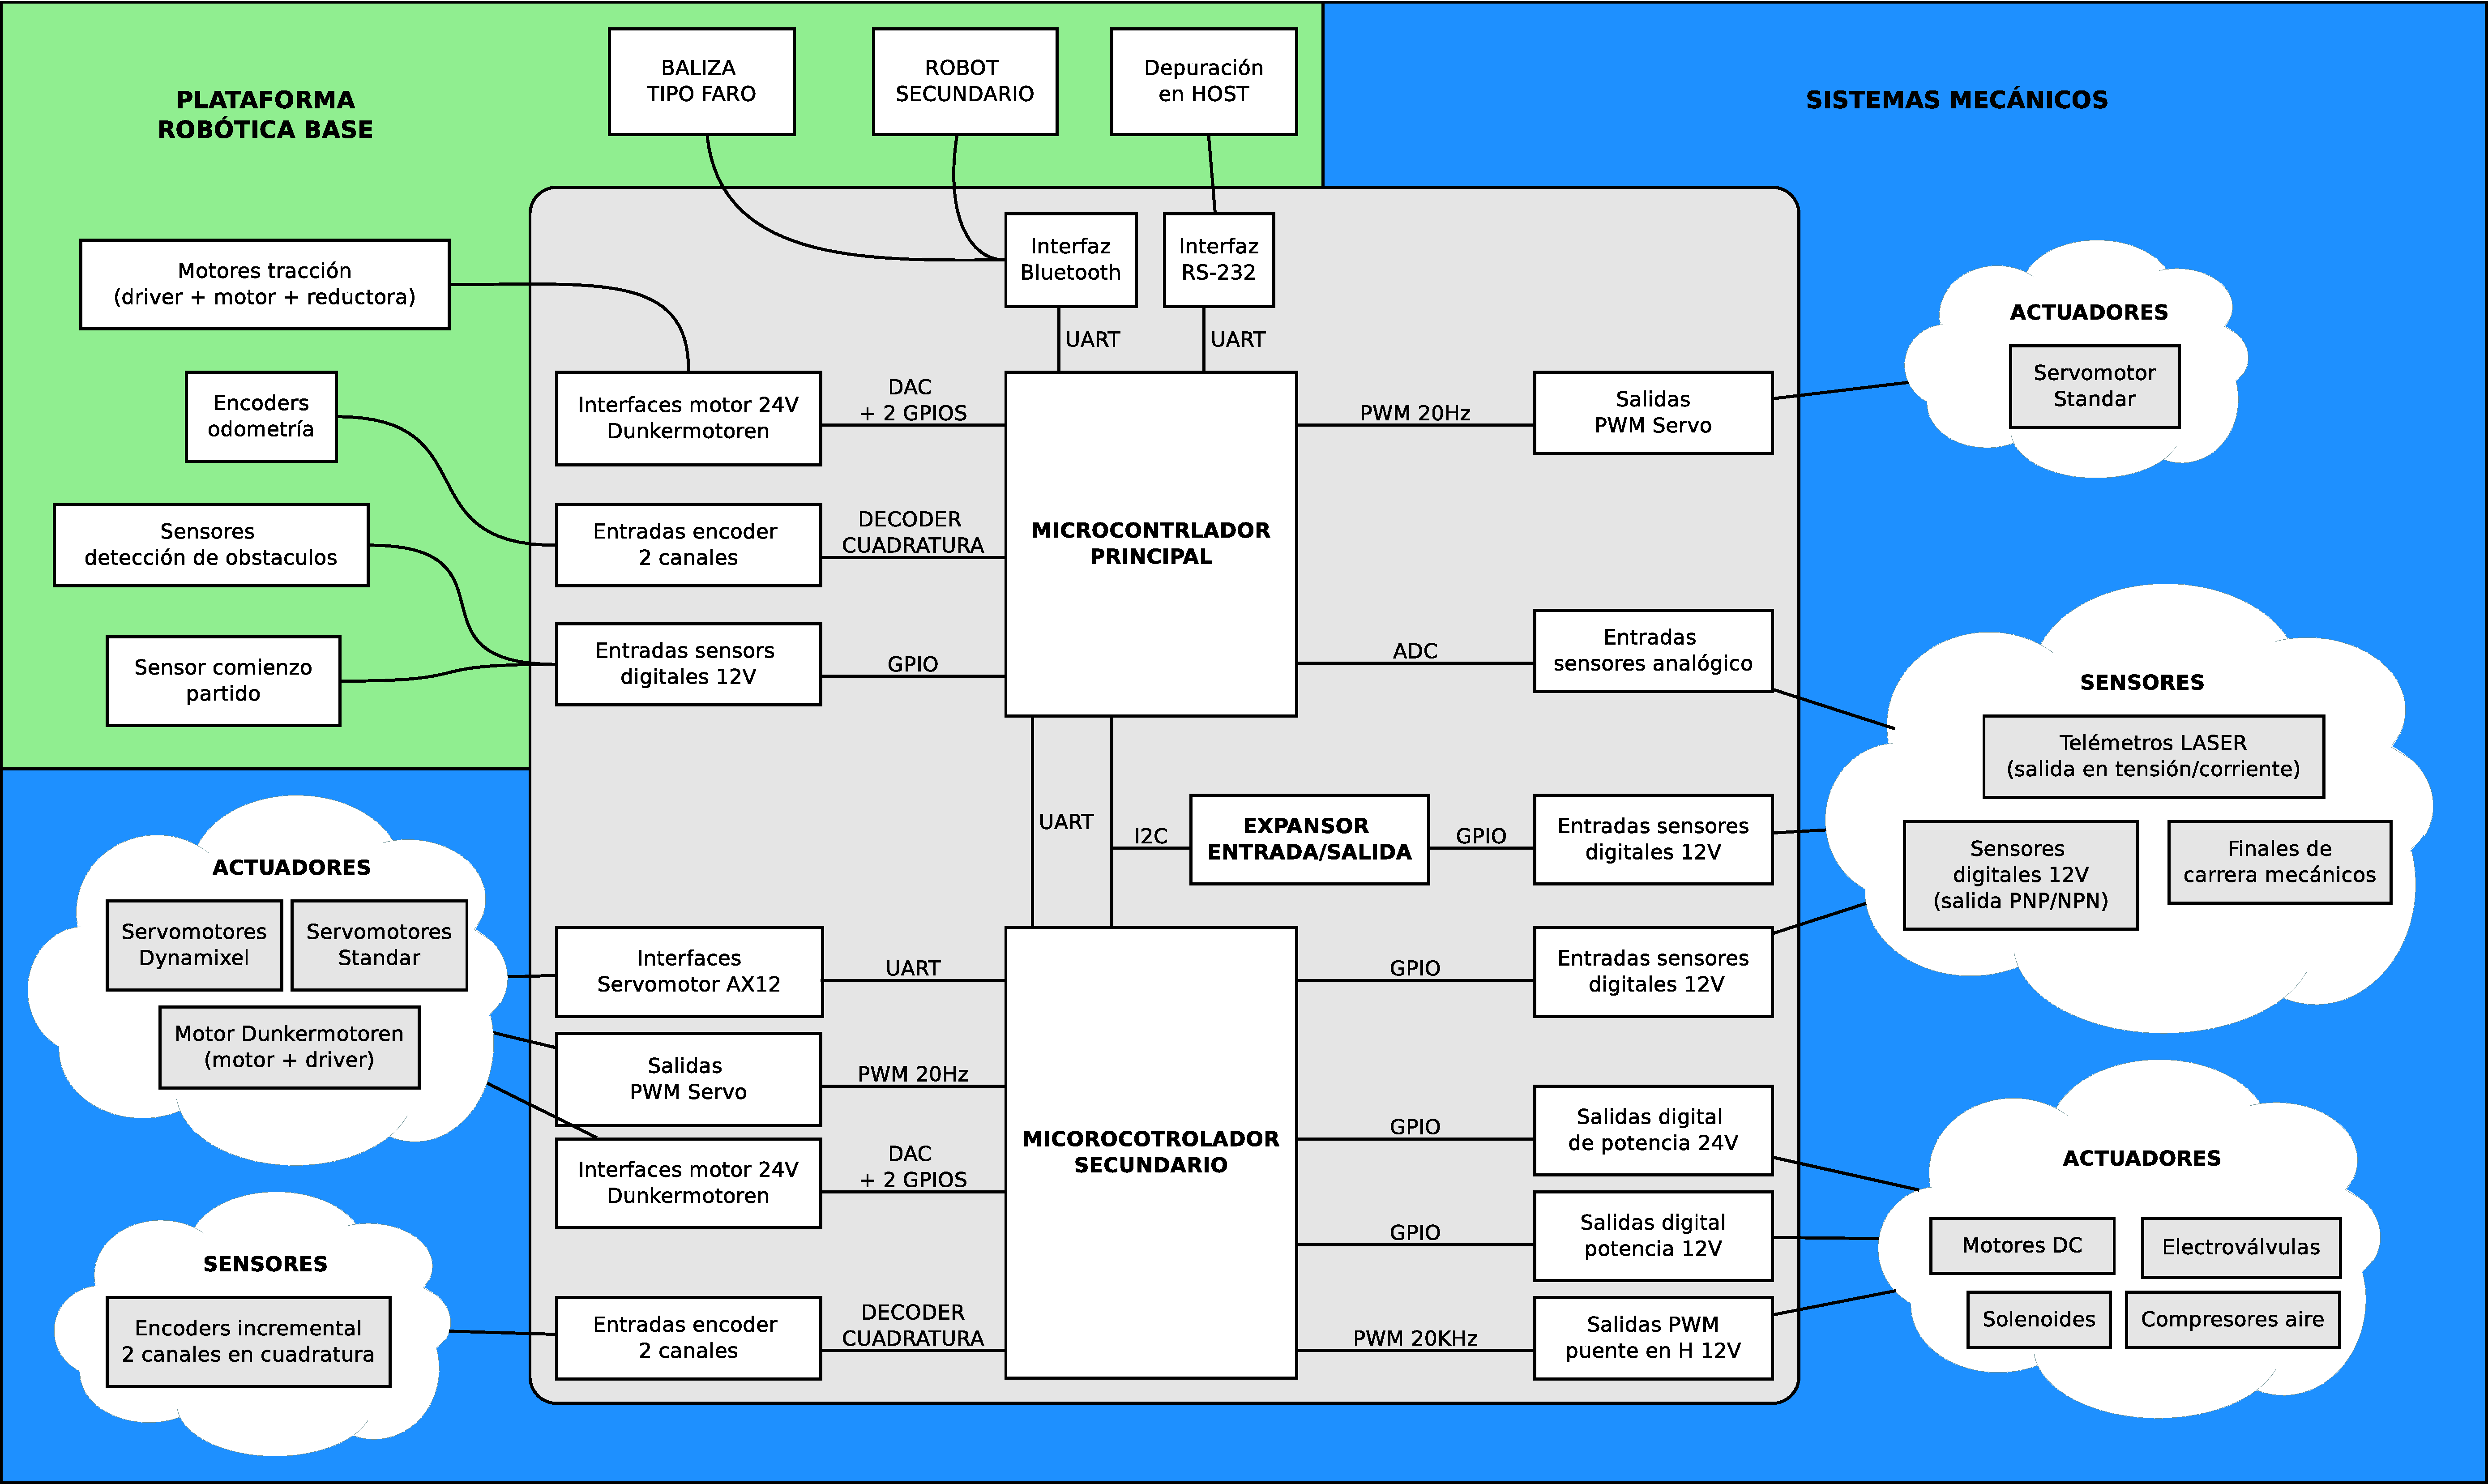
\includegraphics[height=.9\textwidth, angle=90]{hardware_arquitectura}
\caption[]{Arquitectura hardware de a la plataforma rob�tica base}
%\label{fig_hardware_arquitectura}
\end{figure}

\subsection{Sistemas mec�nicos}

\begin{figure}[ht]
\centering
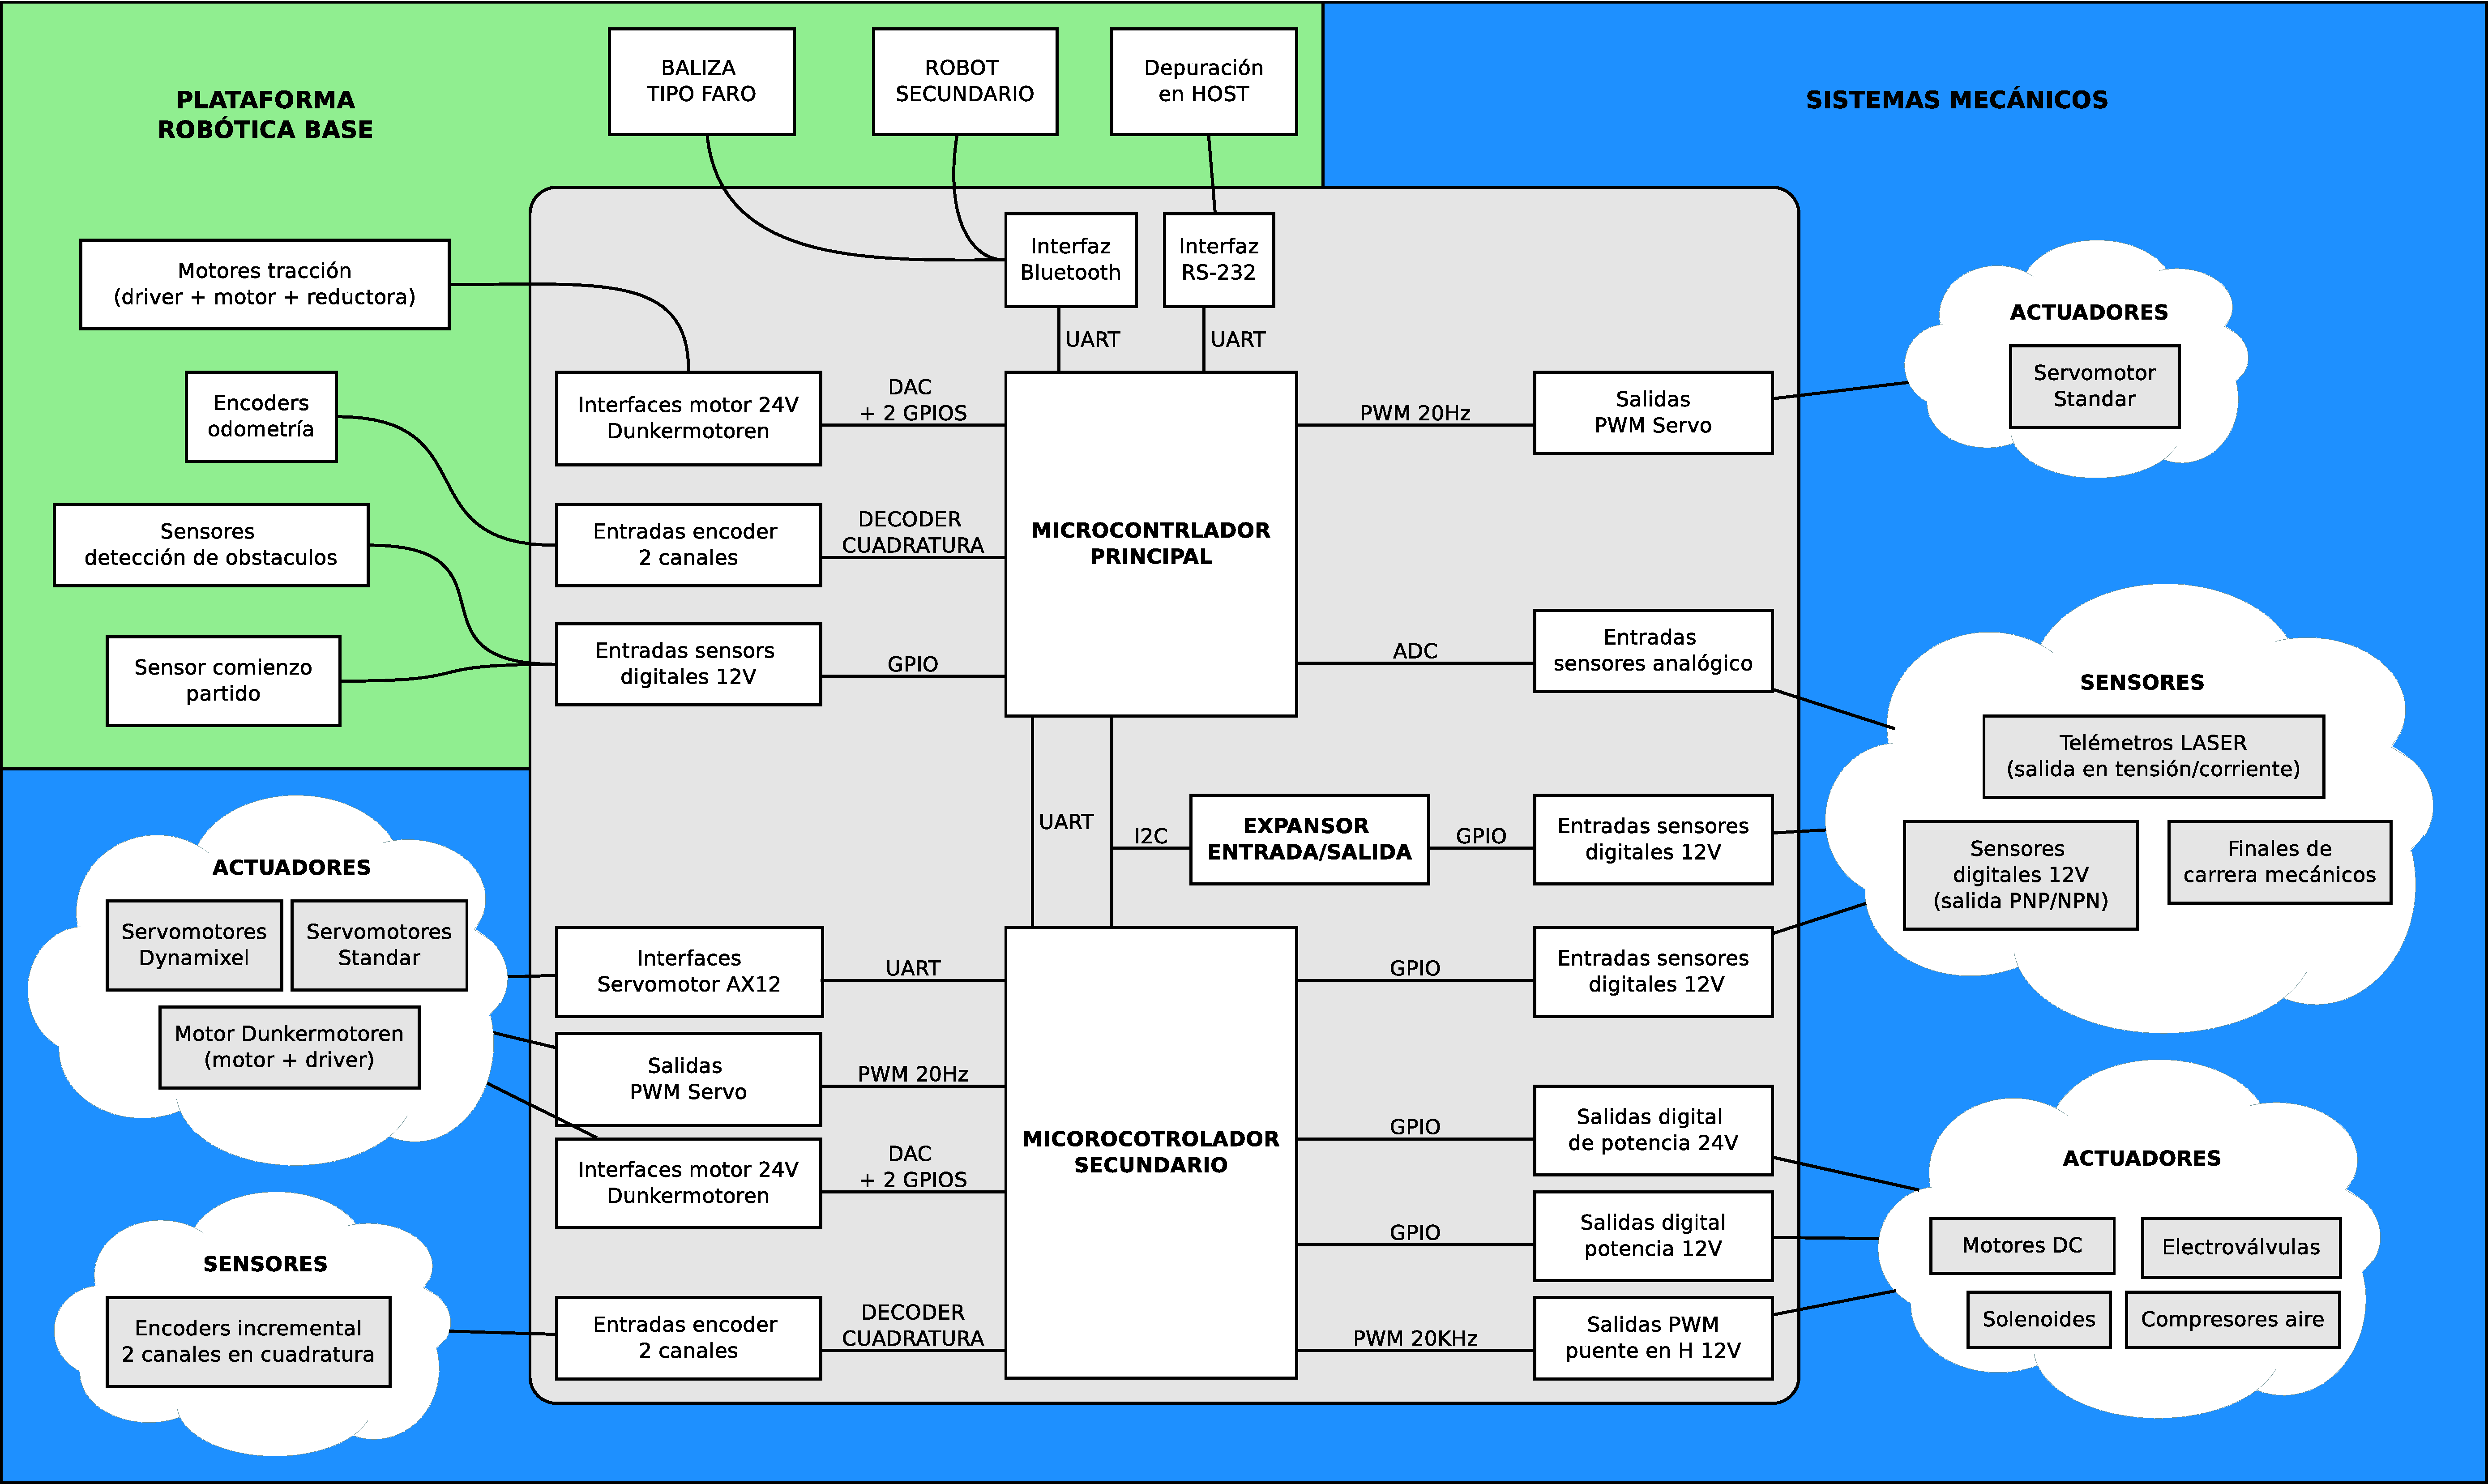
\includegraphics[height=.9\textwidth, angle=90]{hardware_arquitectura}
\caption[]{Arquitectura hardware del robot de Eurobot}
\label{fig_hardware_arquitectura}
\end{figure}

\subsection{�rbol de alimentaci�n}

\begin{figure}[ht]
\centering
%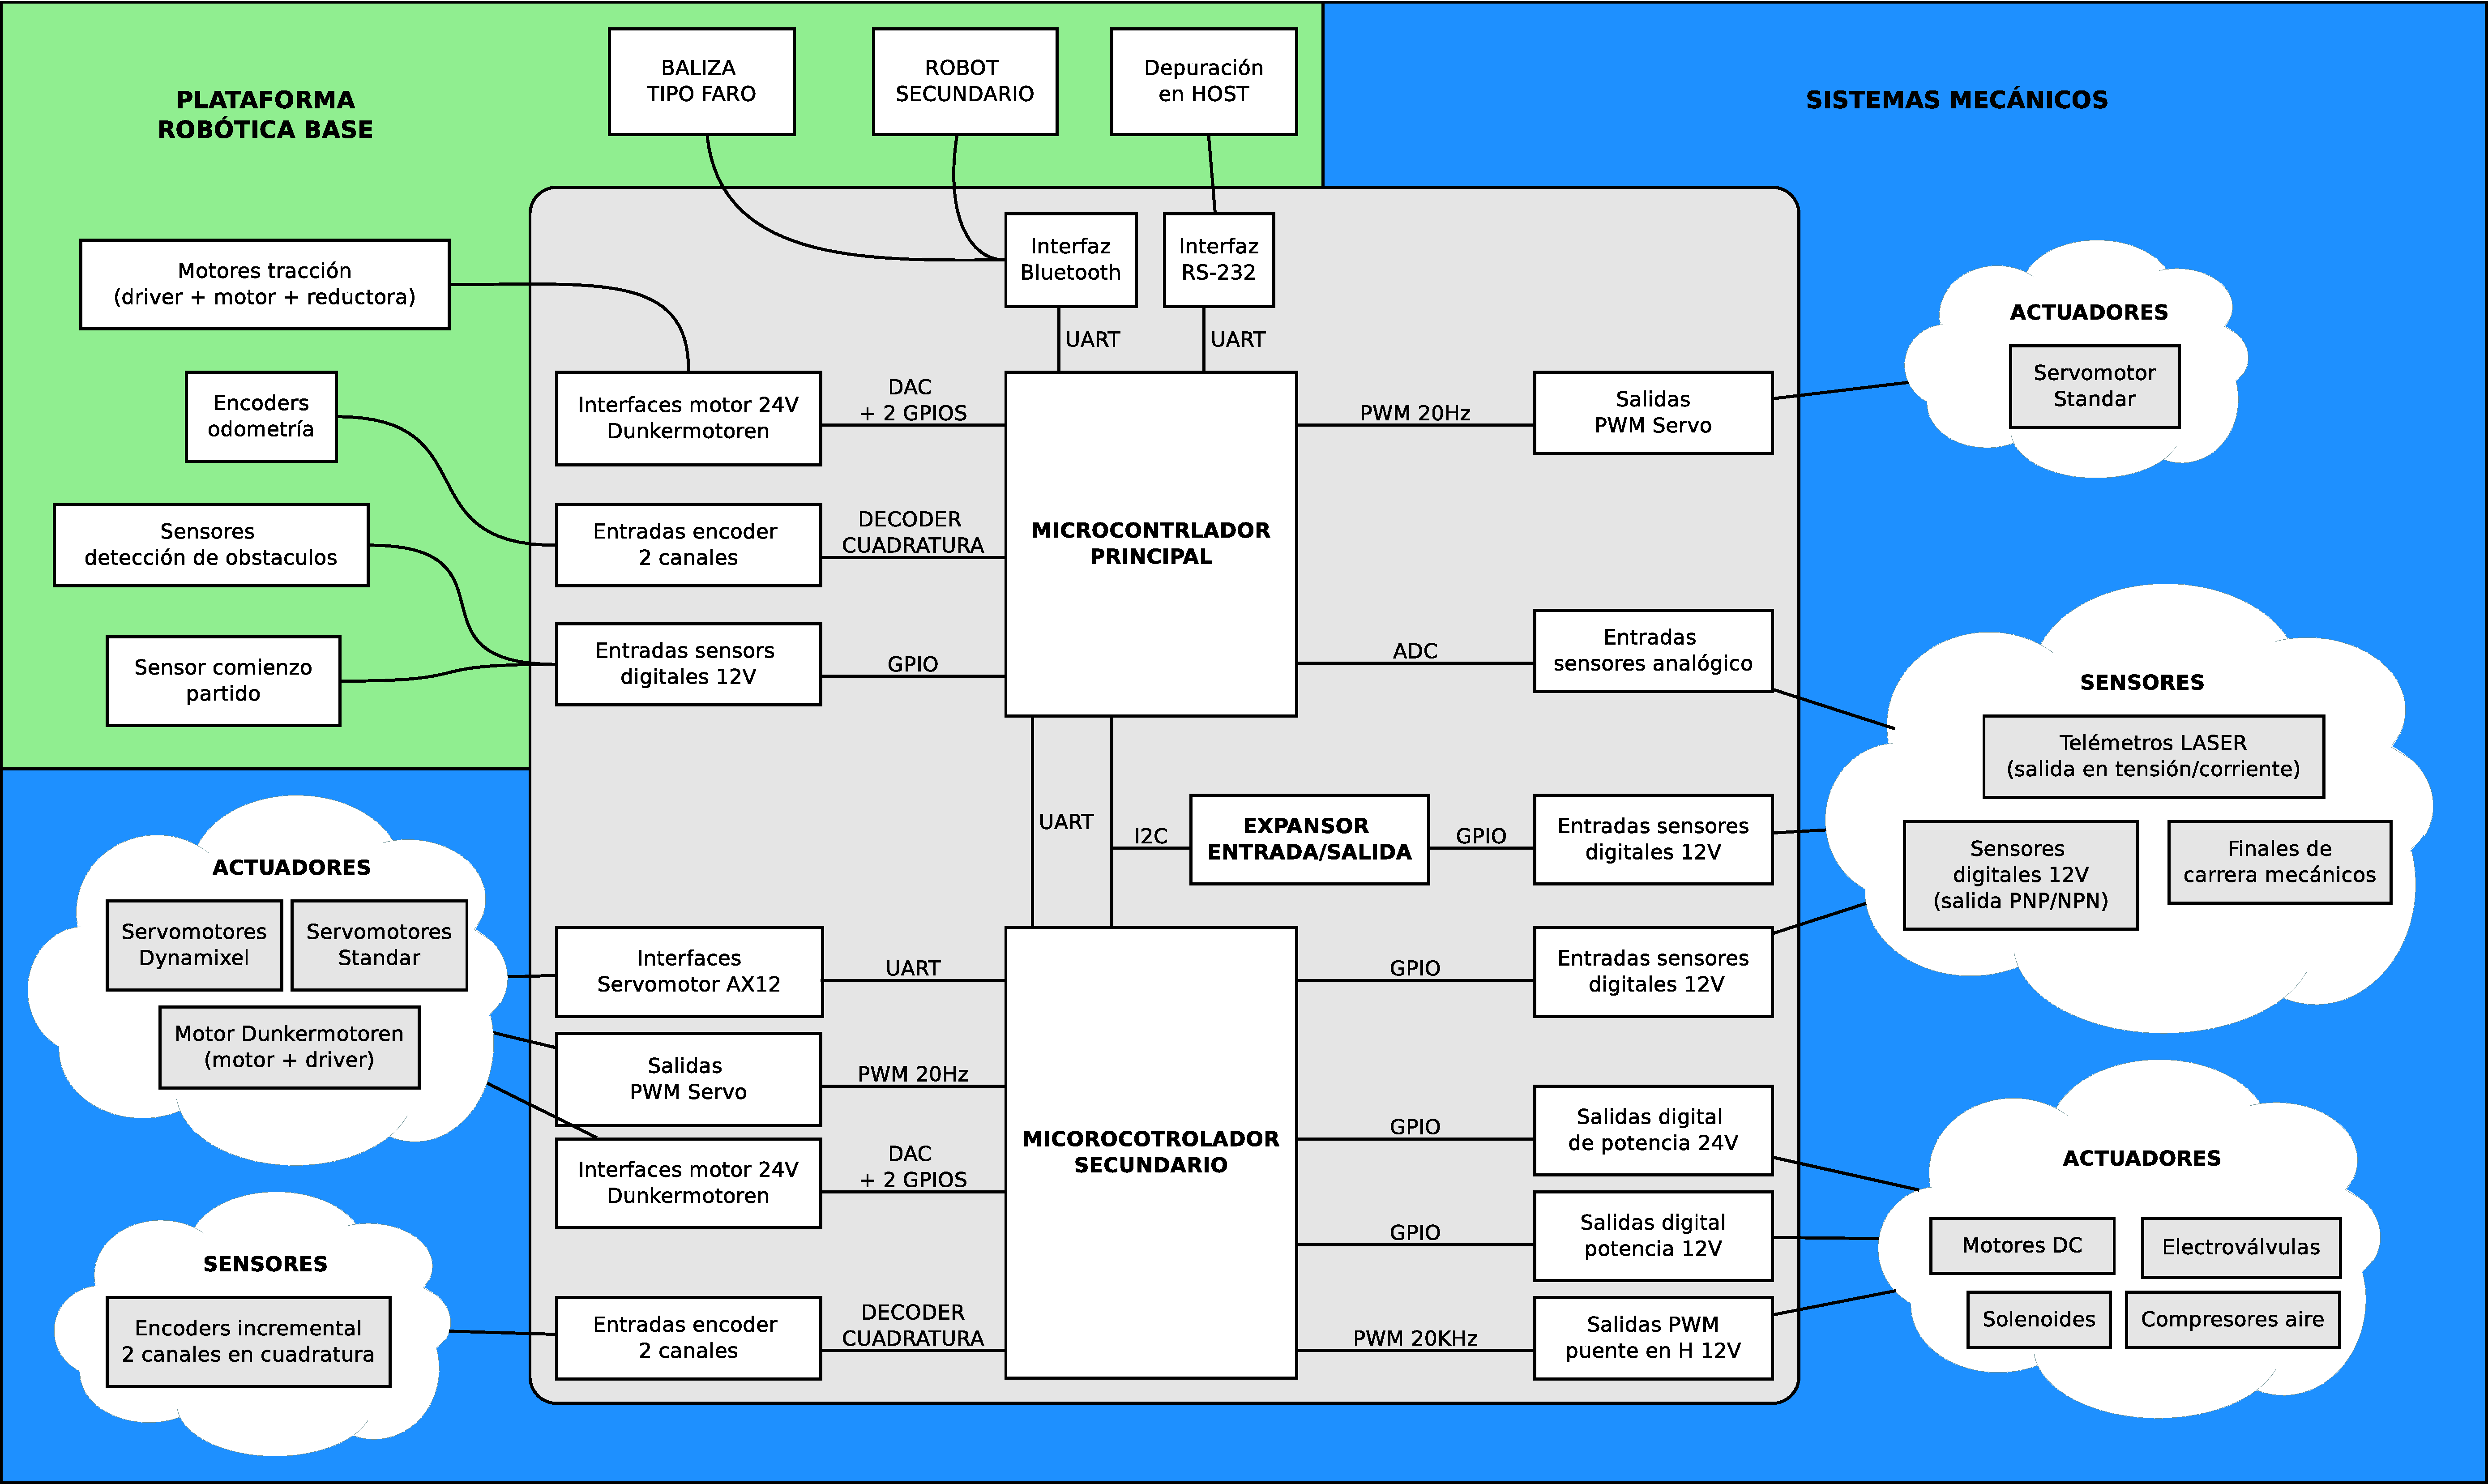
\includegraphics[height=.9\textwidth, angle=90]{hardware_arquitectura}
\caption[]{Arquitectura hardware del �rbol de alimentaci�n del robot de Eurobot}
%\label{fig_hardware_arquitectura}
\end{figure}

\section{Implementaci�n HW del robot principal}
\subsection{Tarjeta principal}
\subsection{Tarjeta de sensores digitales}
\subsection{Tarjeta de actuadores}
\subsection{Tarjeta de control de alimentaci�n}
\subsection{Tarjeta de alimentaci�n}

\section{Implementaci�n HW del robot secundario}



%%% Local Variables:
%%% TeX-master: "../book"
%%% End:
